% cone20-simple.tex

\section{Mach 1.5 flow over a 20-degree cone -- Simple boundaries}
\label{cone20-simple-sec}
%
Let's start with a simple-to-imagine flow of ideal air over a sharp-nose of a supersonic projectile.
Figure\,\ref{cone20-flight-fig} is a reproduction of Fig.\,3 from Maccoll's 1937 paper\,\cite{maccoll_1937a} 
and shows a shadowgraph image of a two-pounder projectile, in flight at Mach 1.576.
We'll restrict our simulation to just the gas flow coming onto and moving up the conical surface 
of the projectile and work in a frame of reference attached to the projectile.
Further, we will assume that all of the interesting features of the flow can be 
The red lines mark out the region of our gas flow simulation, 
assuming axial symmetry about the centreline of the projectile.

\begin{figure}[htbp]
\begin{center}
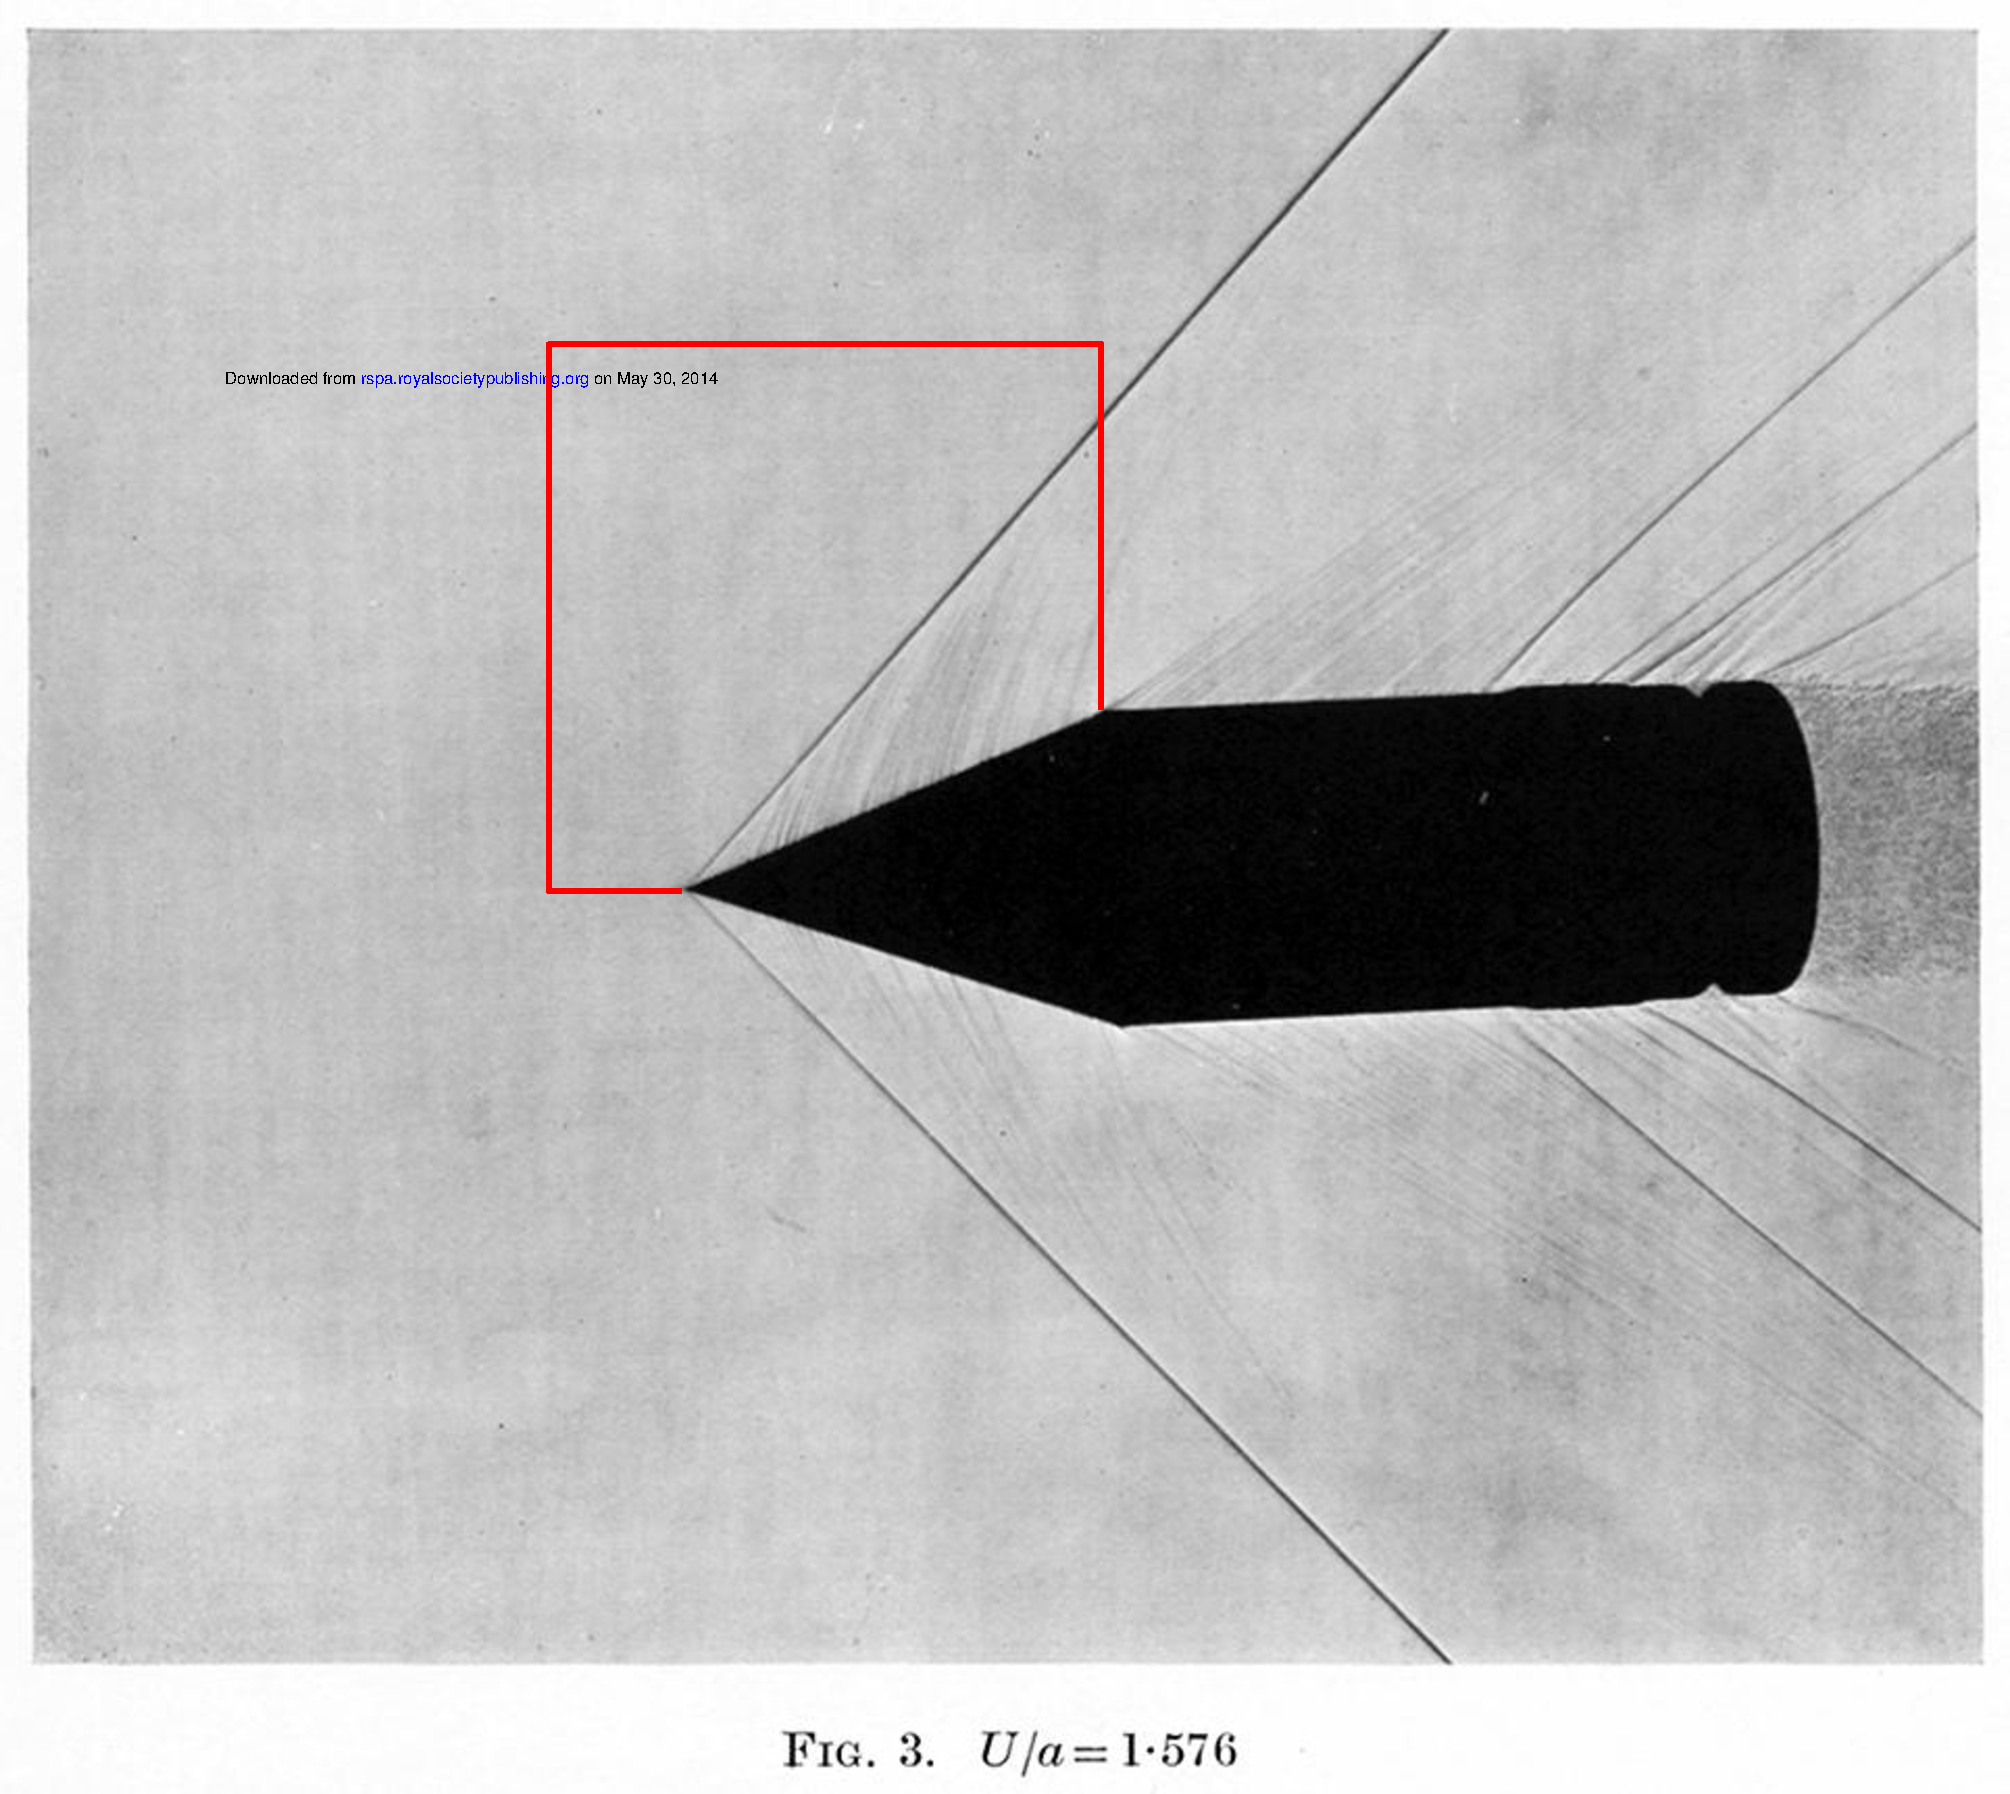
\includegraphics[width=0.9\textwidth, viewport=76 168 949 761, clip=true]{../2D/cone20-simple/maccoll-1937-fig3.pdf}
\end{center}
\caption{A two-pound projectile in flight.  A conical shock is attached to the sharp nose of the projectile. 
	 This photograph was published by Maccoll in 1937.
	 The red lines have been added to demark the region of gas flow for which we will set up our simulation.}
\label{cone20-flight-fig}
\end{figure}

\subsection{Input script (.py)}\index{boundary conditions!set\_BC!example of use}
%
To build our simulation, we abstract the boxed region from Figure\,\ref{cone20-flight-fig}
and consider the axisymmetric flow of an ideal, inviscid gas over a sharp-nosed cone 
with 20 degree half angle.
With the constraint of axisymmetry implies zero angle of incidence for the original 3D flow.

\medskip
The resulting flow, in the steady-state limit, should have a single shock that is 
straight in this 2D meridional plane (but conical in the original 3D space).
The angle of this shock can be checked against Taylor and Maccoll's gas-dynamic theory and,
since the simulation demands few computational resources (in both memory and run time), 
it is useful for checking that the simulation and
plotting programs have been built and installed correctly.

\begin{figure}[htbp]
\begin{center}
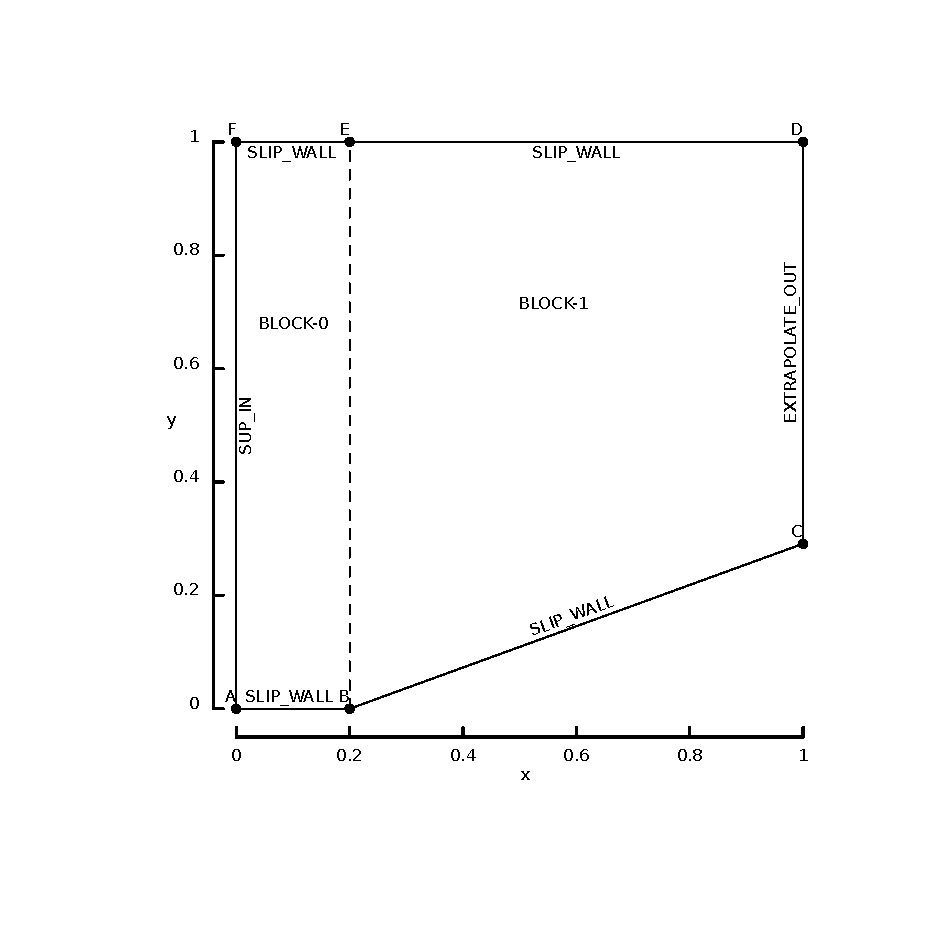
\includegraphics[width=10cm, viewport=76 78 389 398]{../2D/cone20-simple/cone20_svg.pdf}
\end{center}
\caption{Schematic diagram of the geometry for a cone 
         with 20 degree half-angle.
	 This PDF figure was generated from the SVG file with some edits 
	 to move the boundary labels to nicer positions.}
\label{cone20-geometry-fig}
\end{figure}

\noindent\topbar
\lstinputlisting[language={}]{../2D/cone20-simple/cone20.py}
\bottombar

\medskip
Despite Figure\,\ref{cone20-flight-fig} being a good motivator for this simulation,
the free-stream conditions of $p_{\infty} = 95.84$\,kPa, $T_{\infty} = 1103$\,K
and $u_{\infty} = 1000$\,m/s are actually related to the shock-over-ramp test problem
in the original ICASE Report\,\cite{jacobs_91d} and are set to give a Mach number of 1.5.
It is left as an exercise for the reader to run a simulation at Maccoll's value of
Mach number and check that the simulation closely matches the shadowgraph image.


\subsection{Running the simulation}
%
Assuming that you have the program executable files built and
accessible on your system's search \texttt{PATH}, as described in Appendix\,\ref{getting-started-file},
try the following commands:\\
%
\topbar\\
\texttt{\$ cd $\sim$/cfcfd3/examples/eilmer3/2D/cone20-simple/}\\
\texttt{\$ ./cone20\_run.sh}\\
\bottombar\\
%
and, within a minute or so, you should end up with a number of files
with various solution data plotted.
The grid and initial solution are created and the time-evolution of the
flow field is computed for 5\,ms (with 862 time steps being required).
The commands invoke the shell script shown below.
This script, less the commands to generate the plot, could be used as
a template for your own simulation shell scripts.

\noindent \topbar
\lstinputlisting[language={}]{../2D/cone20-simple/cone20_run.sh}
\bottombar

\subsection{Results and Postprocessing}
%
Figure\,\ref{cone20-low-res-fig} shows the flow field 5\,milliseconds after flow start.
This has been long enough for the flow to reach a steady state, with the shock being essentially straight.
The plots have been produced with \verb!Paraview!, picking up the \verb!plot/cone20.pvd! file.
The time stamp in the lower left corner has been added as an \verb!Annotate Time Filter!, 
selected from the main \verb!Filters! menu.
Also, the pressure field has been plotted as a coloured \verb!surface!, 
while the temperature field has been plotted as a \verb!surface with edges!
to clearly show the computational grid.
The distortion of the grid in the right-hand block is a result of the area-orthogonality (AO) grid generator
making the compromises required to achieve a reasonably-orthogonal mesh at the edges of the block.
The default transfinite grid generator would have produced a mesh that appears less distorted
overall but would have individual cells that are more sheared for this particular block.
For the rectangular block on the left, both generators would produce the same mesh.

\begin{figure}[htbp]
\begin{center}
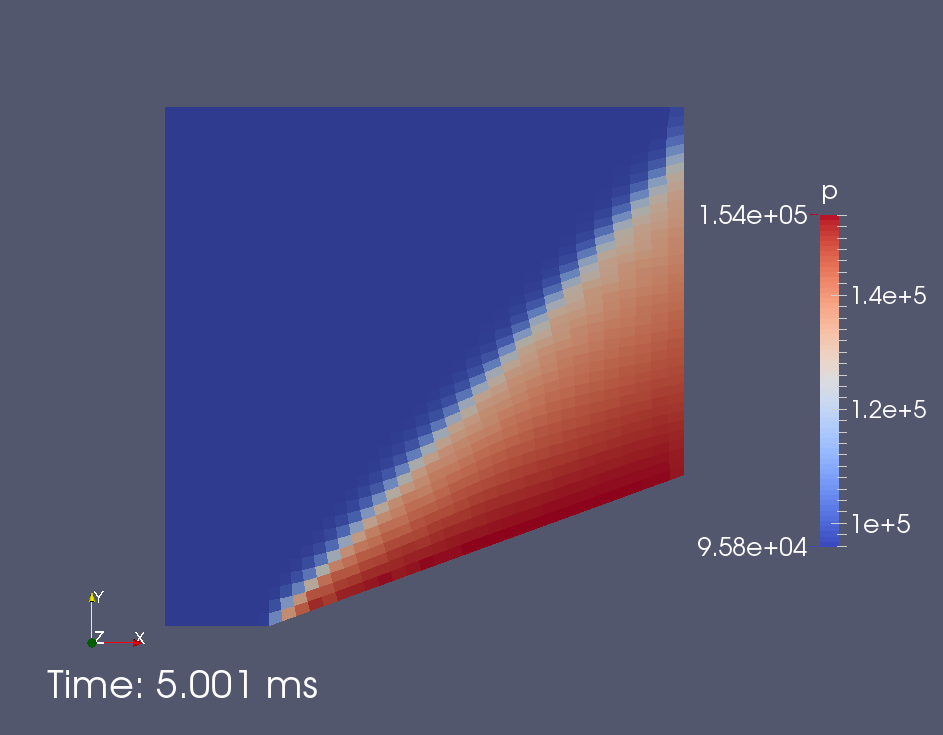
\includegraphics[width=0.45\textwidth]{../2D/cone20-simple/cone20_p.png}
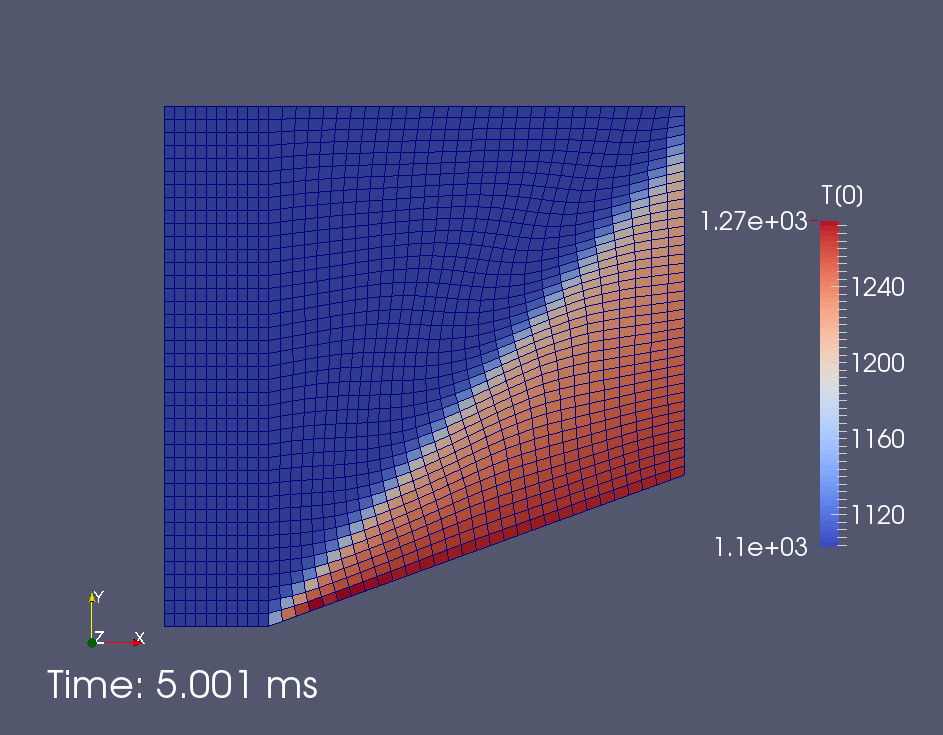
\includegraphics[width=0.45\textwidth]{../2D/cone20-simple/cone20_T0_with-mesh.png}
\end{center}
\caption{Pressure and temperature fields for a low-resolution simulation 
         of flow over a cone with 20 degree half-angle.
         The temperature field plot also included the mesh.}
\label{cone20-low-res-fig}
\end{figure}

% \begin{figure}[htbp]
% \begin{center}
% 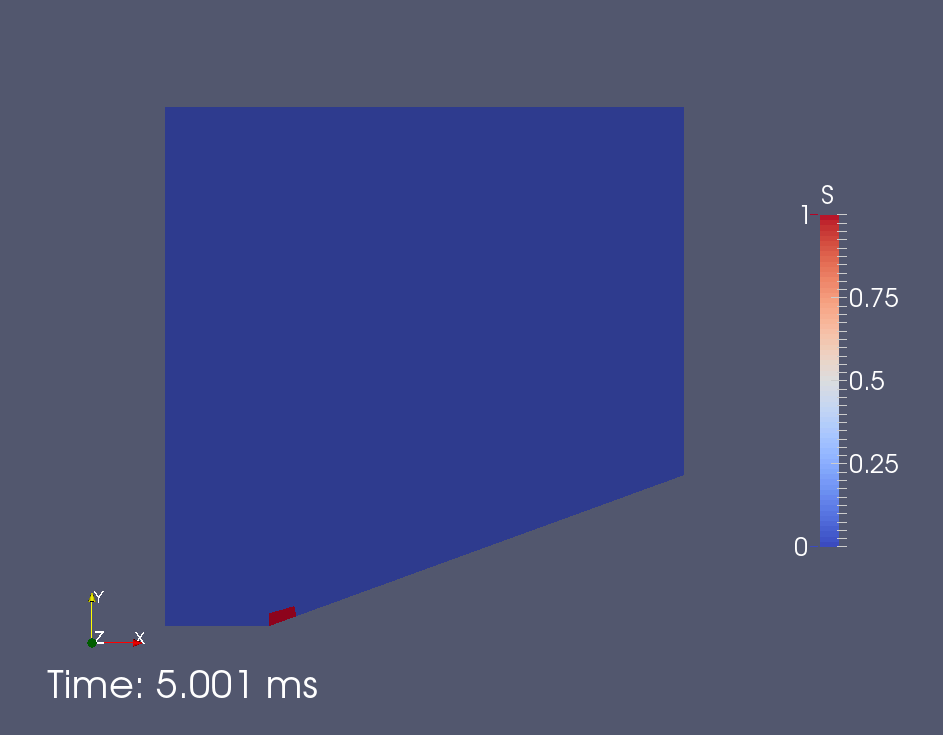
\includegraphics[width=0.8\textwidth]{../2D/cone20-simple/cone20_S.png}
% \end{center}
% \caption{Shock-sensor data for flow over a cone with 20 degree half-angle.
%          For the \texttt{adaptive} flux calculator, 
% 	 this sensor indicates the regions
%	 of the flow where the more dissipative scheme should be used.}
% \label{cone20-shock-sensor-fig}
% \end{figure}

\medskip
The shock displayed in the pressure field shows features that are characteristic 
of a flow solution produced by a ``shock-capturing'' code such as \verb!Eilmer3!.
With the coarse grid, the shock has a stair-case appearance.
This is accentuated by the plotting program which was set to display 
the cell-average value as a uniform colour within each cell.
Also, when following a line that crosses the shock,
a small number of cells to be counted before the full pressure jump has been reached.
In an ideal, inviscid simulation, the shock should be a zero-thickness transition.
This can be approached by increasing the mesh resolution, as seen in Figure\,\ref{cone20-high-res-fig}.
The high-resolution solution is looking clean but the computational cost, in terms of time, 
has gone up from a few seconds to nearly 2 hours.

\begin{figure}[htbp]
\begin{center}
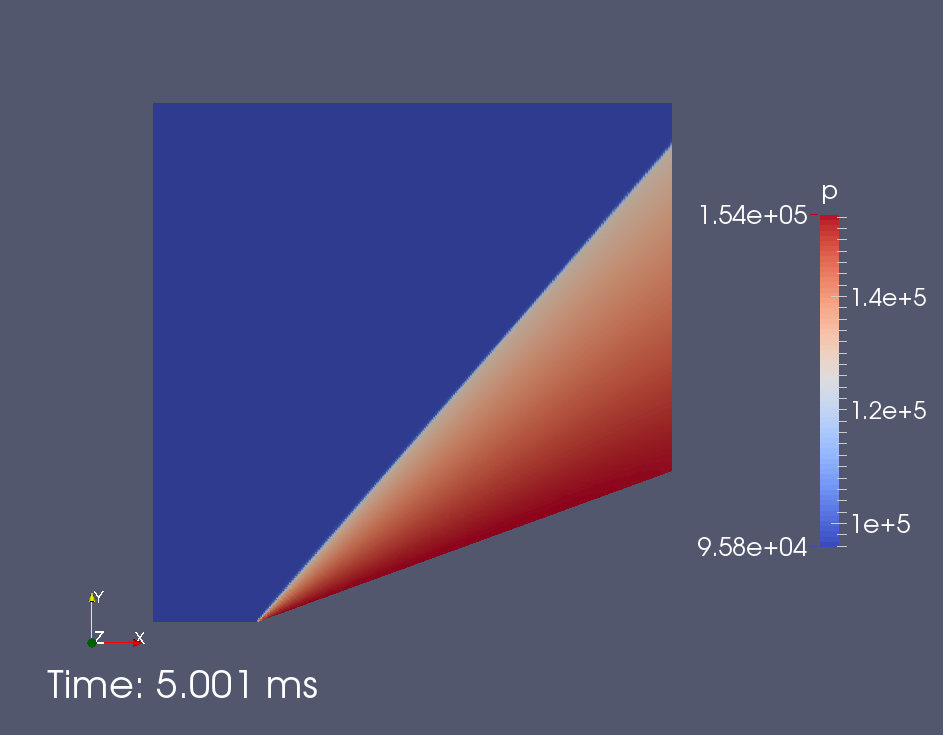
\includegraphics[width=0.45\textwidth]{../2D/cone20-simple/cone20_p_factor-8-grid-res.png}
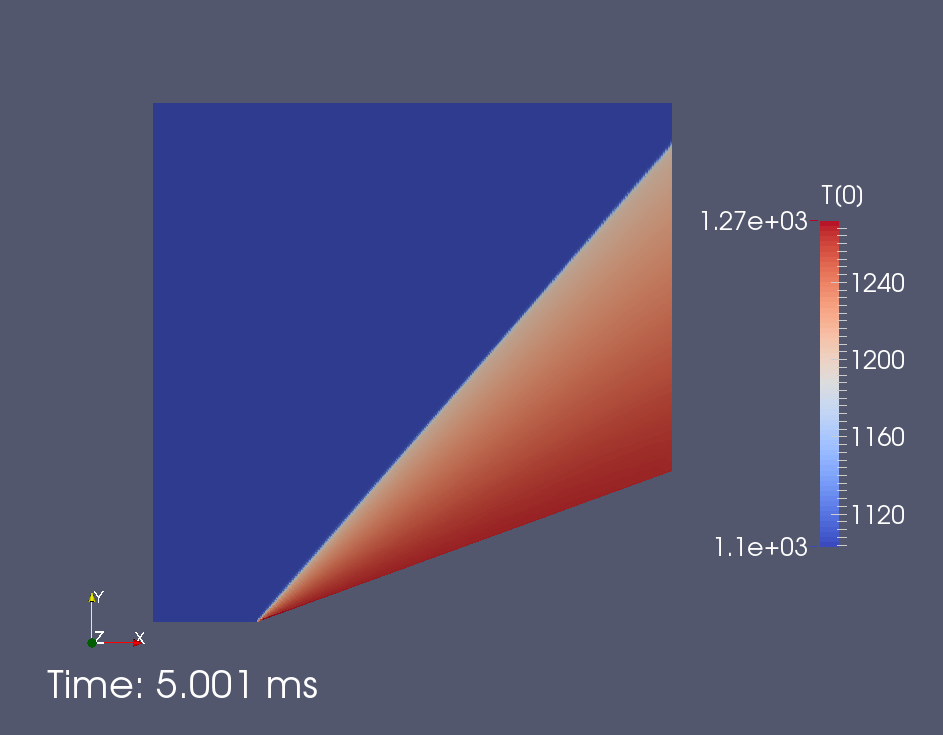
\includegraphics[width=0.45\textwidth]{../2D/cone20-simple/cone20_T0_factor-8-grid-res.png}
\end{center}
\caption{Pressure and temperature fields for a mesh with 8 times more resolution in each direction.}
\label{cone20-high-res-fig}
\end{figure}

\medskip
From Chart 5 in Ref.\,\cite{ames_53}, the expected steady-state shock wave
angle is 49$^o$ and, from Chart 6, the pressure coefficient is
$$
\frac{p_{cone-surface} - p_{\infty}}{q_{\infty}} \approx 0.387
$$
and the dynamic pressure for the specified free stream is
$q_{\infty} = \frac{1}{2} \rho_{\infty} u_{\infty}^2 \approx 151.38$\,kPa.
Figure~\ref{cone20-axial-force-fig} shows the pressure coefficient 
estimated as
$$
C_p = \frac{f_x - p_{\infty} A}{q_{\infty} A}
$$
from the simulated axial force, $f_x$, written into the simulation log file
and frontal area of the cone, $A$.

\begin{figure}[htbp]
\begin{center}
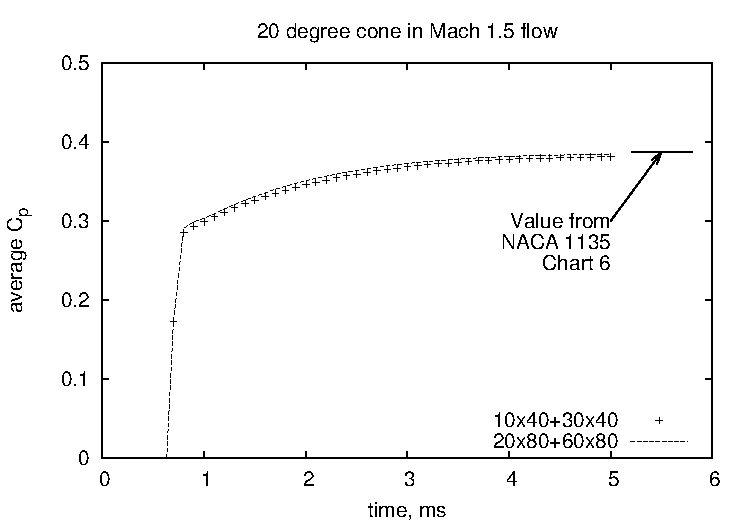
\includegraphics[width=10cm]{../2D/cone20-simple/cone20_cp.pdf}
\end{center}
\caption{Evolution of the axial (drag) force
         for flow over a cone with 20 degree half-angle
	 for two mesh resolutions.}
\label{cone20-axial-force-fig}
\end{figure}

\medskip
Beyond the usual slice-and-dice type of postprocessing that is provided by \verb!e3post.py!, 
it may be useful to do specialized calculations on the flow data.
In this flow, the shock is expected to be straight and we can compute
that it should have an angle of $\beta = 48.96^o$, with respect to the free-stream direction,
using one of the gas-dynamic functions from \verb!cfpylib!: 
\begin{verbatim}
from cfpylib.gasdyn.ideal_gas_flow import beta_cone
from math import degrees, radians
beta = beta_cone(V1=1000.0, p1=95.84e3, T1=1103.0, theta=radians(20.0))
print "beta=", degrees(beta), "degrees"
\end{verbatim}

The \texttt{estimate\_shock\_angle.py} script uses the Python code libraries 
that the \texttt{e3post.py} is built upon to pick up the data, 
locate the shock position along each strip of cells in the x-direction,
and then fit a straight line to the collected points.
Note that the points from the top right of the flow solution are omitted from the straight-line fit
because the top boundary has interfered with the flow.
The shock points and the fitted line are shown in Fig.\ref{cone20-shock-points-fig} 

\begin{figure}[htbp]
\begin{center}
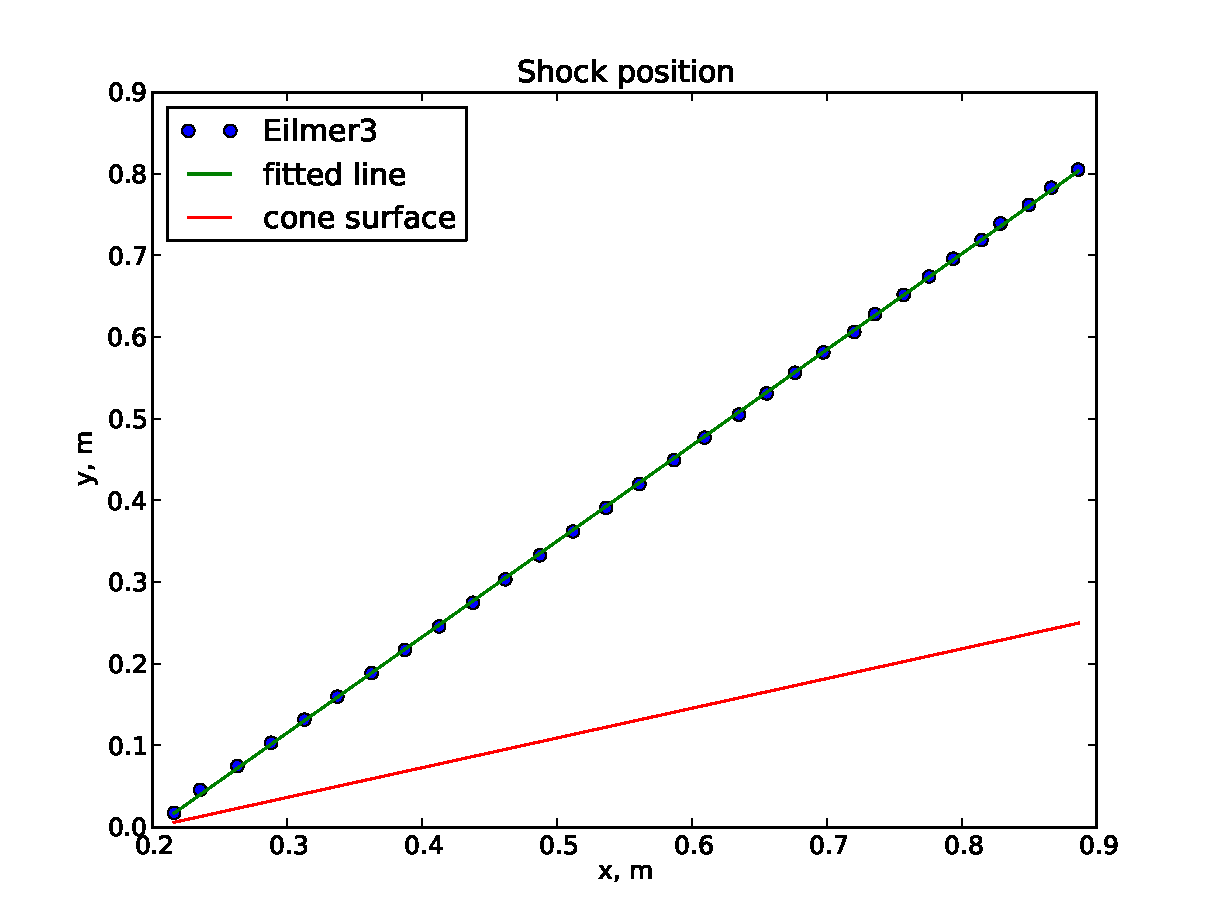
\includegraphics[width=10cm]{../2D/cone20-simple/shock-shape.pdf}
\end{center}
\caption{Shock shape for Mach 1.5 flow over the 20-degree cone.}
\label{cone20-shock-points-fig}
\end{figure}

The script below uses the data reading and storage capability provided by 
the class \texttt{StructuredGridFlow}, which is imported from \texttt{e3\_flow.py}.
Given a file containing the flow data for a block of cells, this class has a \texttt{read} 
method that picks up the data.
The flow and position data is stored in a dictionary, with one multidimensional numpy array 
for each variable.
Access to the pressure in cell \texttt{i,j,k} of block \texttt{ib,jb} is achieved by
putting these indices together as \texttt{blockData[ib][jb].data['p'][i,j,k]}.
The core of the data handling is in the function \texttt{locate\_shock\_front()}
in the middle of the script.

\noindent
\topbar
\lstinputlisting[language={}]{../2D/cone20-simple/estimate_shock_angle.py}
\bottombar

\subsection{Notes}
\begin{itemize}
\item Remember that long-format command-line options start with two dashes.
      For example \texttt{--job=cone20}.
      These double dashes are a little hard to distinguish in the shell
      scripts.

\item Run time is approximately 17 seconds for 862 steps on a computer with 
      an AMD Phenom II X4 840, 800\,MHz processor.
      Of course, the shared-memory code does not make use of the other 4 processor cores,
      however, there is an MPI version of the code that can.

\item This cone20.py file really has full access to the Python interpreter
      on your system.  Later examples will show how to use Python to write
      data files from within the input script.  Be careful.

\item Python is a dynamic language.
      It is easy to bind names to new objects within your script.
      Be careful that you do not rebind essential names that will be
      later used by the \texttt{e3prep.py} program.
      Where this might happen in a non-obvious way is in the importing
      of foreign modules (to do something interesting in your script)
      with the command ``from \textit{module-name} import *''.

\item Awk script for extracting x-force data from the simulation log file.
      New users might like to use an equivalent program written in Python.
      \lstinputlisting[language={}]{../2D/cone20-simple/cp.awk}\index{xforce\_list!example of use}

\item The script \texttt{cone20\_run\_mpi.sh} is available for running the simulation
  with the parallel version of the code on a machine with OpenMPI installed.
  This script is essentially the same as shown for the shared-memory simulation
  with the MPI simulation being started with the commands:\index{e3mpi.exe!example of use}
\begin{verbatim}
mpirun -np 2 e3mpi.exe -f cone20 --run
\end{verbatim}
  The only other modification required is to look for the surface-force data in the
  log file \texttt{e3mpi.0001.log} rather than \texttt{e3shared.log}.

\end{itemize}
